
\subsection{Data description}

The potential amount of news related to sustainable development is enormous. Thousands are published every day around the globe. In order to assess what drives the financial markets and their impact on a broad portfolio, we need a large database with frequent updates. When conducting an event study, many researchers compose their database by either collecting events from archives or utilizing an existing database of comprehensive and carefully selected events. As both approaches involve using a database of hand-picked events, their observations updates infrequently, hence the data and the results are not useful in practice. \\
In this study I use a data set provided by Matter. The company has developed a systematic collection of daily news articles from more than 150.000 media sources, which measure the amount of times a specific company has been mentioned positively, negatively, or neutrally in relation to a specific SDG or on broad level in news articles worldwide.   
The data set is updated every day at midnight and uses artificial intelligence to relate every single news article to more than 75.000 publicly traded companies. 

Consequently, the relevant events analyzed in this paper are not specified from the data set. Instead, I apply a rule-based approach to detect large spikes in news articles for individual companies. The short term analysis applies daily observations, and identifies an event as a one standard deviation move away from the mean of daily articles. The methodology produces 1.046 negative events from 155 distinct companies and 3.565 positive events from 212 companies from January 2018 to January 2023.  





\subsection{Estimation methodology}



\subsection{Short term abnormal returns in the Market Model} \label{ST_results}

With a baseline in the thesis' theoretical and methodological groundwork from prior sections, the following presents the main empirical results in relation to the hypotheses. Initially, the individual subsections depict the specific hypothesis that are relevant for the given subsection.  
To test hypothesis #1 and #2 of whether negative and positive SDG-related events impacts firm value on the short term, I separate negative and positive events and assess the aggregated development in abnormal returns 10 days before and 10 days after an event has occurred. Moreover, I isolate the effect of the individual SDGs to test hypothesis #a of #1 and #2 of whether events related to specific sustainability goals are more relevant for investors than other. The Market Model is applied to measure abnormal returns around an event. All returns in this section are value-weighted by market capitalization.    

\subsubsection{Negative news} \label{sec: st_negative}

The average abnormal returns and development in cumulative average abnormal returns, inferred from the Market Model, are illustrated in figure \ref{fig:ST_neg_news}. To support the analysis, the AAR and CAAR are portrayed along with their respective 95\% confidence intervals and the amount of events on a given day relative to the event day $(t = 0)$ (right axis) illustrated by the barplot in the background. 

The left y-axis depicts the abnormal return and the x-axis is the number of days before and after an event has occurred. The average effect on returns from negative events is represented by the blue line in the graph. 

Focusing on negative news, the sample average abnormal returns of the event date at $(t=0)$ is significantly negative at -0.36\% at a 1\% level. Investors are reacting to spikes in bad news of firms by selling their shares. The days following an event demonstrates no abnormal performance. The effect of the news appear to be priced in earlier than the spike in news occurs. 

The effect is approximately zero on average until $t = -5$ upon which the AAR decreases in the days leading up to the event date. The only significantly negative AARs are found at $t=-5$ and between $t=-2$ to $t=0$ at a $5\%$ level.  Nonetheless, the CAAR is significantly negative from $t=-5$ and through the remaining window where it bottoms at approximately $1.5\%$ 10 days after an event. 
The declining nature of the CAAR suggests that the market gradually learns about the negative events upon which the prospective events are gradually priced in. After the spike in news on the event date the news has limited impact. \\ 


\begin{figure} [H]
    \centering
    \caption{Negative news: AAR and CAAR}
    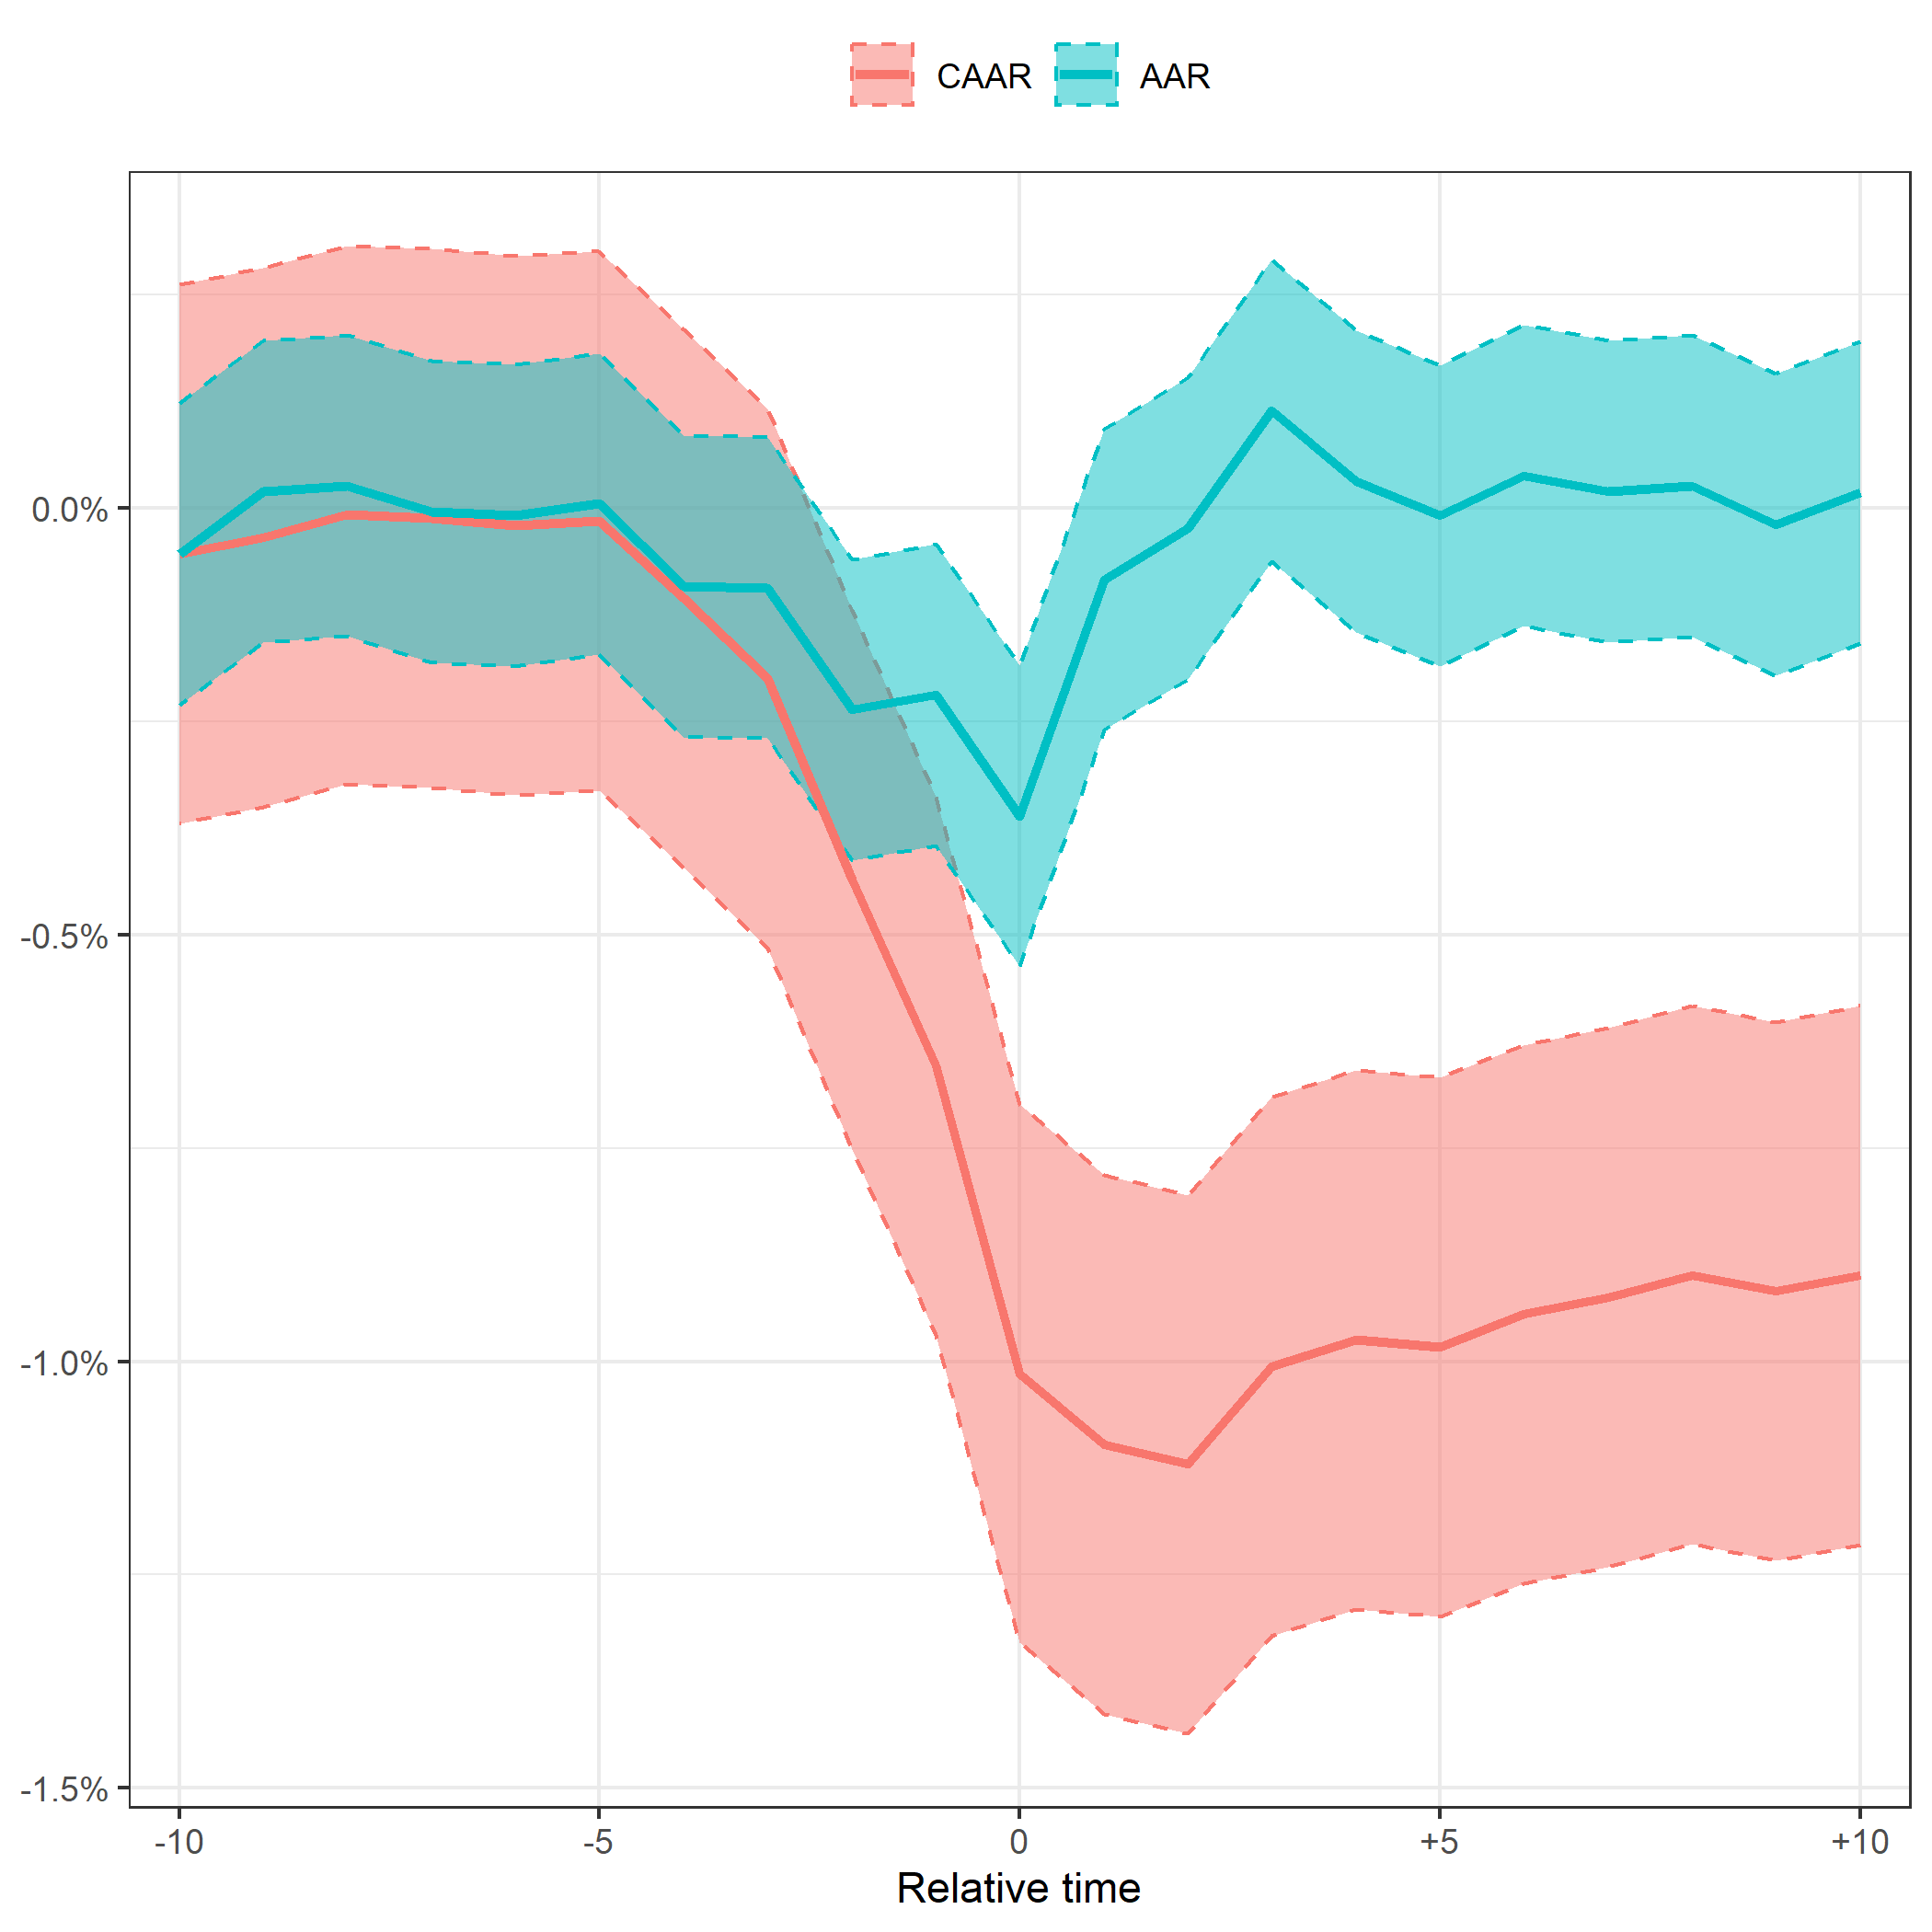
\includegraphics[scale=0.6]{Projekt/1.Figures analysis/ST_negative_all_CI.png}
     \caption*{\footnotesize The figure illustrates the average abnormal return (AAR) and cumulative AAR (CAAR) around the event date (t = 0) of negative news. The lines (left axis) represent the average and the ribbons represent the 95th confidence intervals. The bars (right axis) represent the amount of events on a given day relative to t = 0. }
    \label{fig:ST_neg_news}
\end{figure} 

 
The barchart in the background offer insights into the extent of media attention in the days around a spike in news. For example, at $t = -1$ the average firm is mentioned approximately 0.5 times the amount of the $t = 0$ day. The bars increase in the days from $t=-5$ to the event date, and at the same time the AAR begins to decline, which imply a relation between attention towards negative news and pessimistic investor behavior even before the event date. 

The selection method for negative events was proposed to gather cases of severe negative abnormal returns. These results are an initial indication of the relation between negative news and investor reactions. However, the method may be late to pick up the signal of negative events or new information on the market.  


\noindent \textbf{Split news on relation to SDGs.} Investigating the abnormal returns associated with news specific to the individual SDGs can potentially deepen the understanding of which themes within corporate sustainability that investors place most emphasis with. However, splitting the data into 17 groups impose a natural restriction on the amount of observations of each group, which generate statistical uncertainty. For example, SDG 4 and 9 only has, respectively, 16 and 83 observations. The results are illustrated in the appendix \ref{fig:ST_neg_bar_all}. With a low amount of observations the CAAR at $t = 10$ associated with each SDG becomes highly insignificant, as indicated by the confidence intervals. To counter the issue I combine the SDGs into five groups known officially as the Five Pillars of SDG. They consist of People, Prosperity, Planet, Peace, and Partnership. The analysis changes focus from the individual SDGs to broader themes within sustainability, which, regardless, allows to adequately test the hypothesis.

\begin{figure} [H]
    \centering
    \caption{SDG 5 pillars: negative news}
    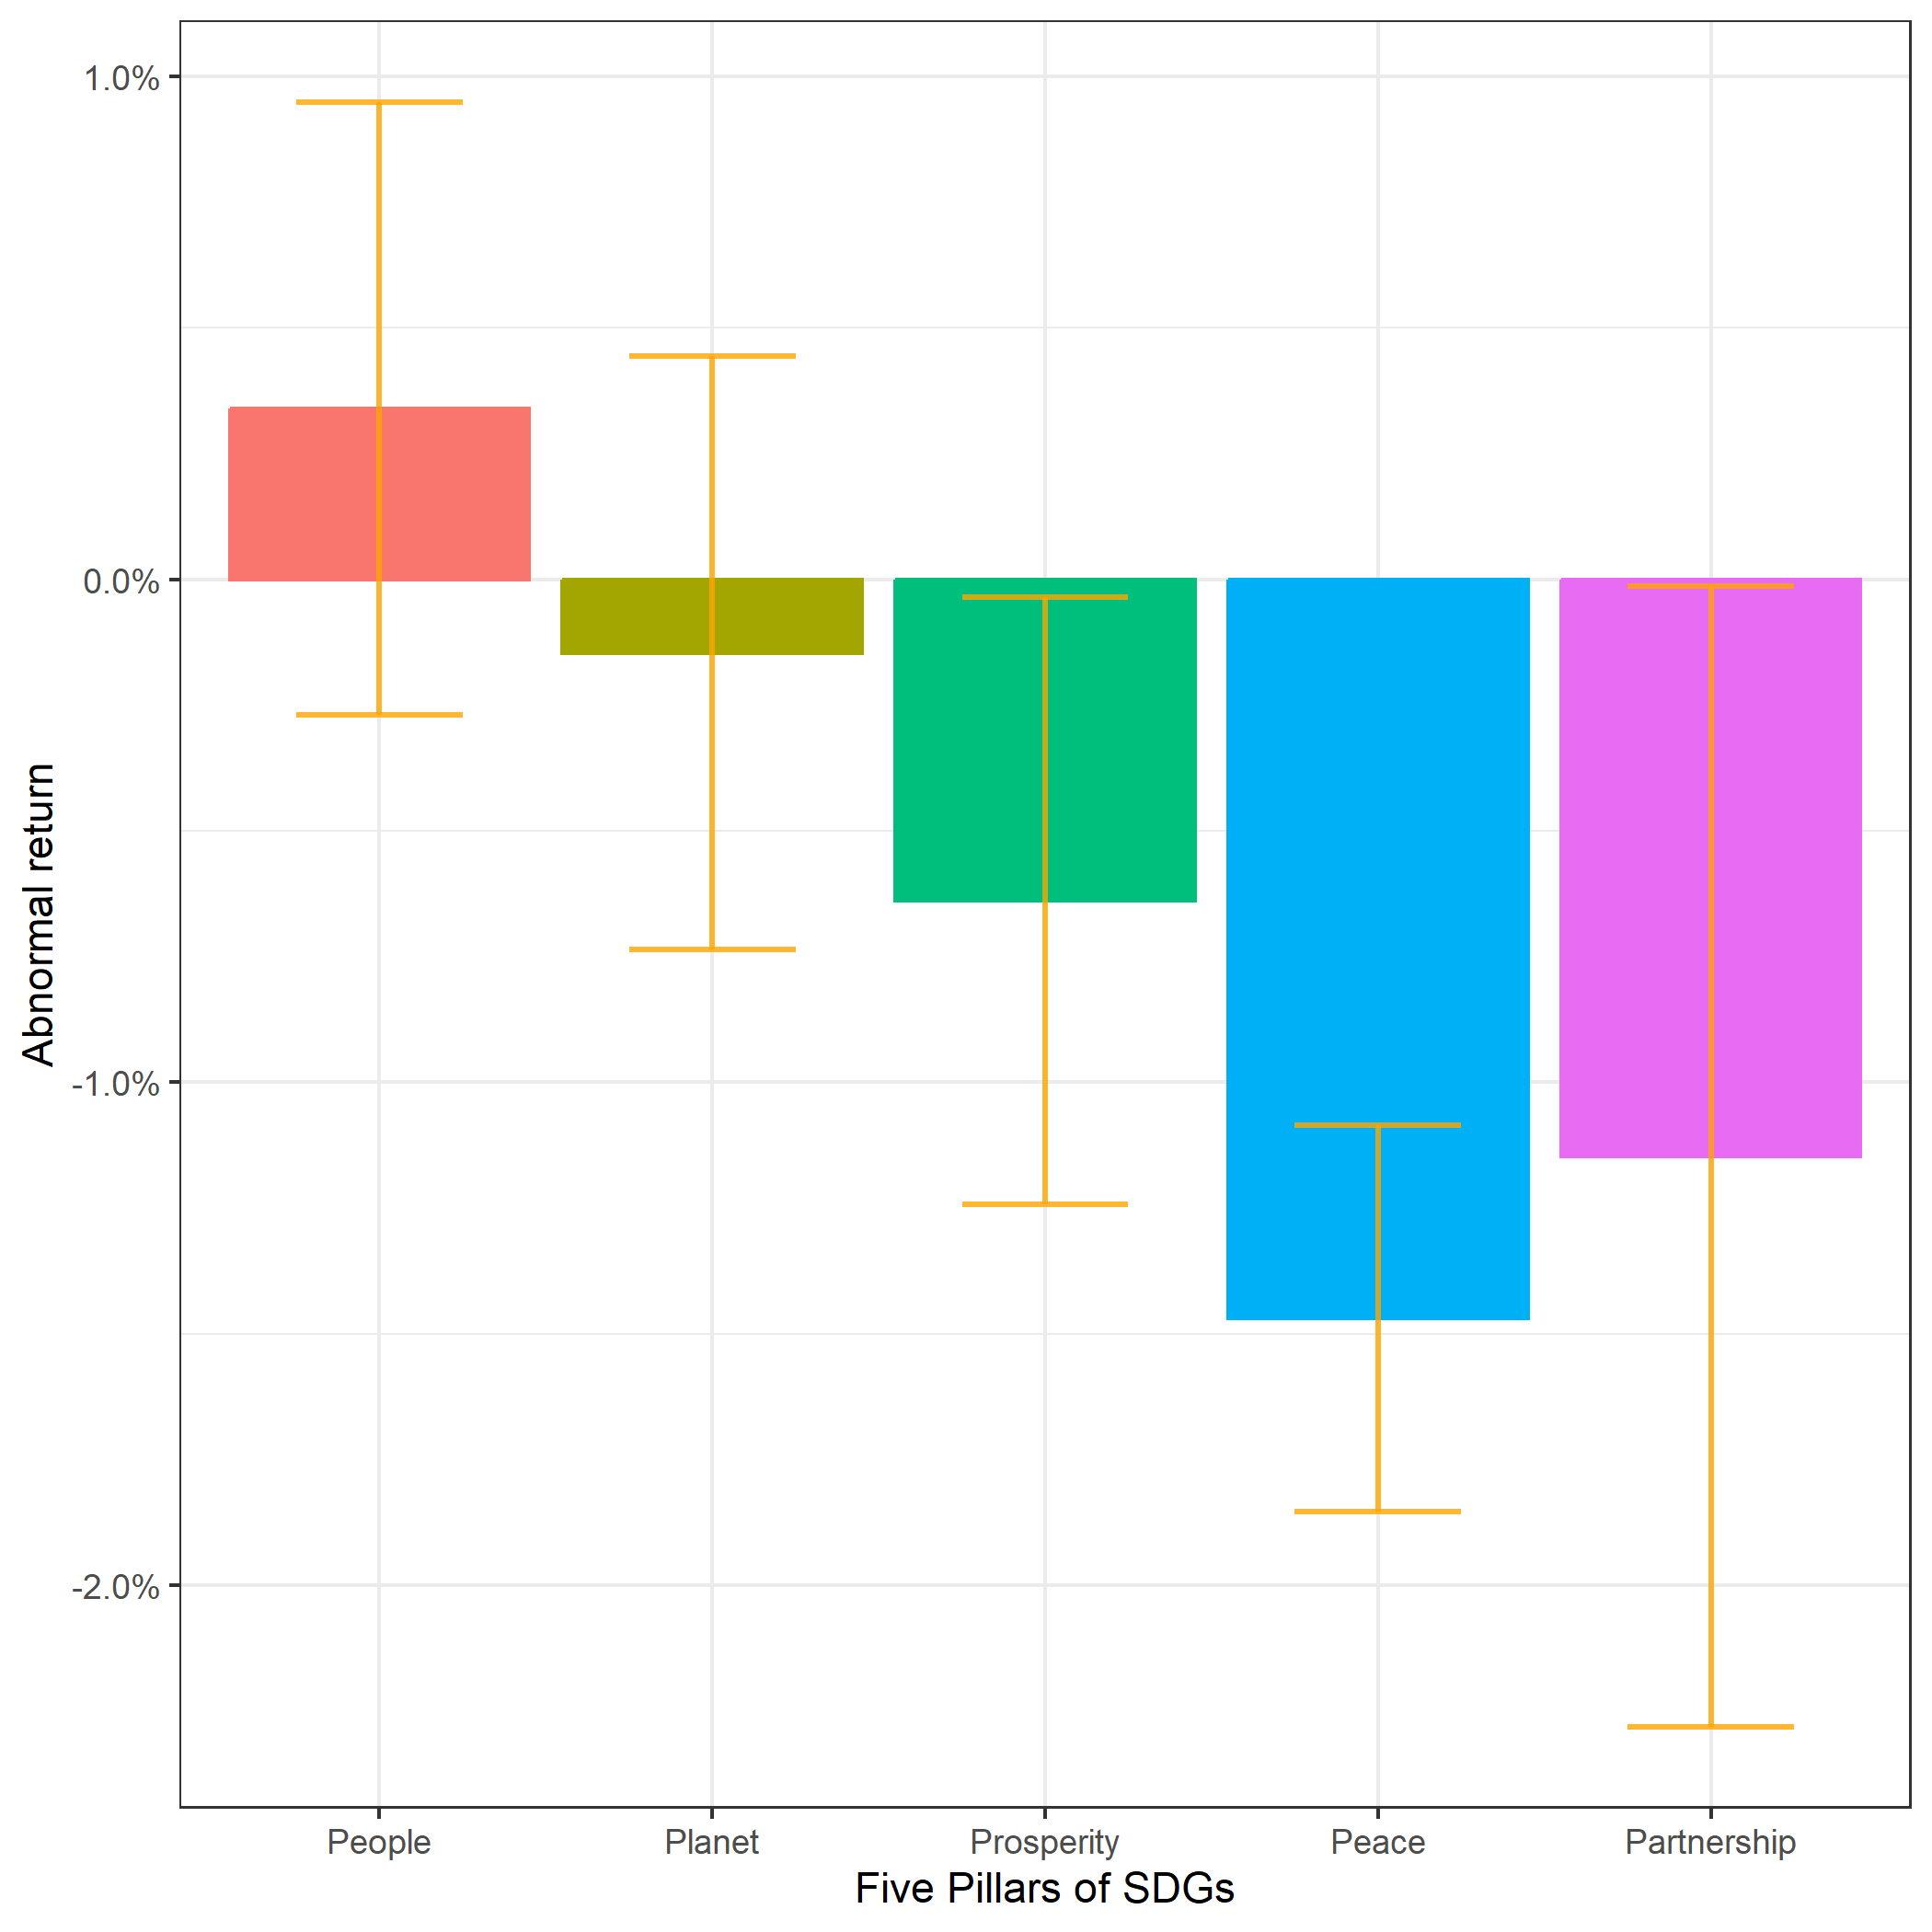
\includegraphics[scale=0.6]{Projekt/1.Figures analysis/ST_negative_sdg_bar_groups_0.png}
    \caption*{\footnotesize The figure illustrates the CAAR on $t = 10$ (the full period) from negative news. The error bars represent the 95\% confidence intervals of the CAAR.}
    \label{fig:ST_neg_bar}
\end{figure}


Figure \ref{fig:ST_neg_bar} illustrate CAAR over the full event window from negative news related to the Five Pillars of SDGs, and indicates that all groups but People are associated with negative abnormal returns. Moreover Prosperity, Peace, and Partnership are associated with significantly negative CAAR.      

\noindent \textbf{Split firms on ESG rating.} 

It is of similar interest to determine whether the sustainability profile of a firm influences how investors react to news related to the social development goals. 

Figure \ref{fig:ST_neg_ESG} employs the same setup as figure \ref{fig:ST_neg_news} and displays the CAAR of event firms with a partition on ESG risk profiles. "Low" represent that a firm has a low risk of encountering complications in relation to ESG affairs. Intuitively, firms with low ESG risks are expected to experience less disputes related to sustainability. Hence, if they do appear in such disputes, a logical reaction from investors would be of more severe magnitude. 

\begin{figure} [H]
    \centering
    \caption{Negative news: CAAR split on ESG rating}
    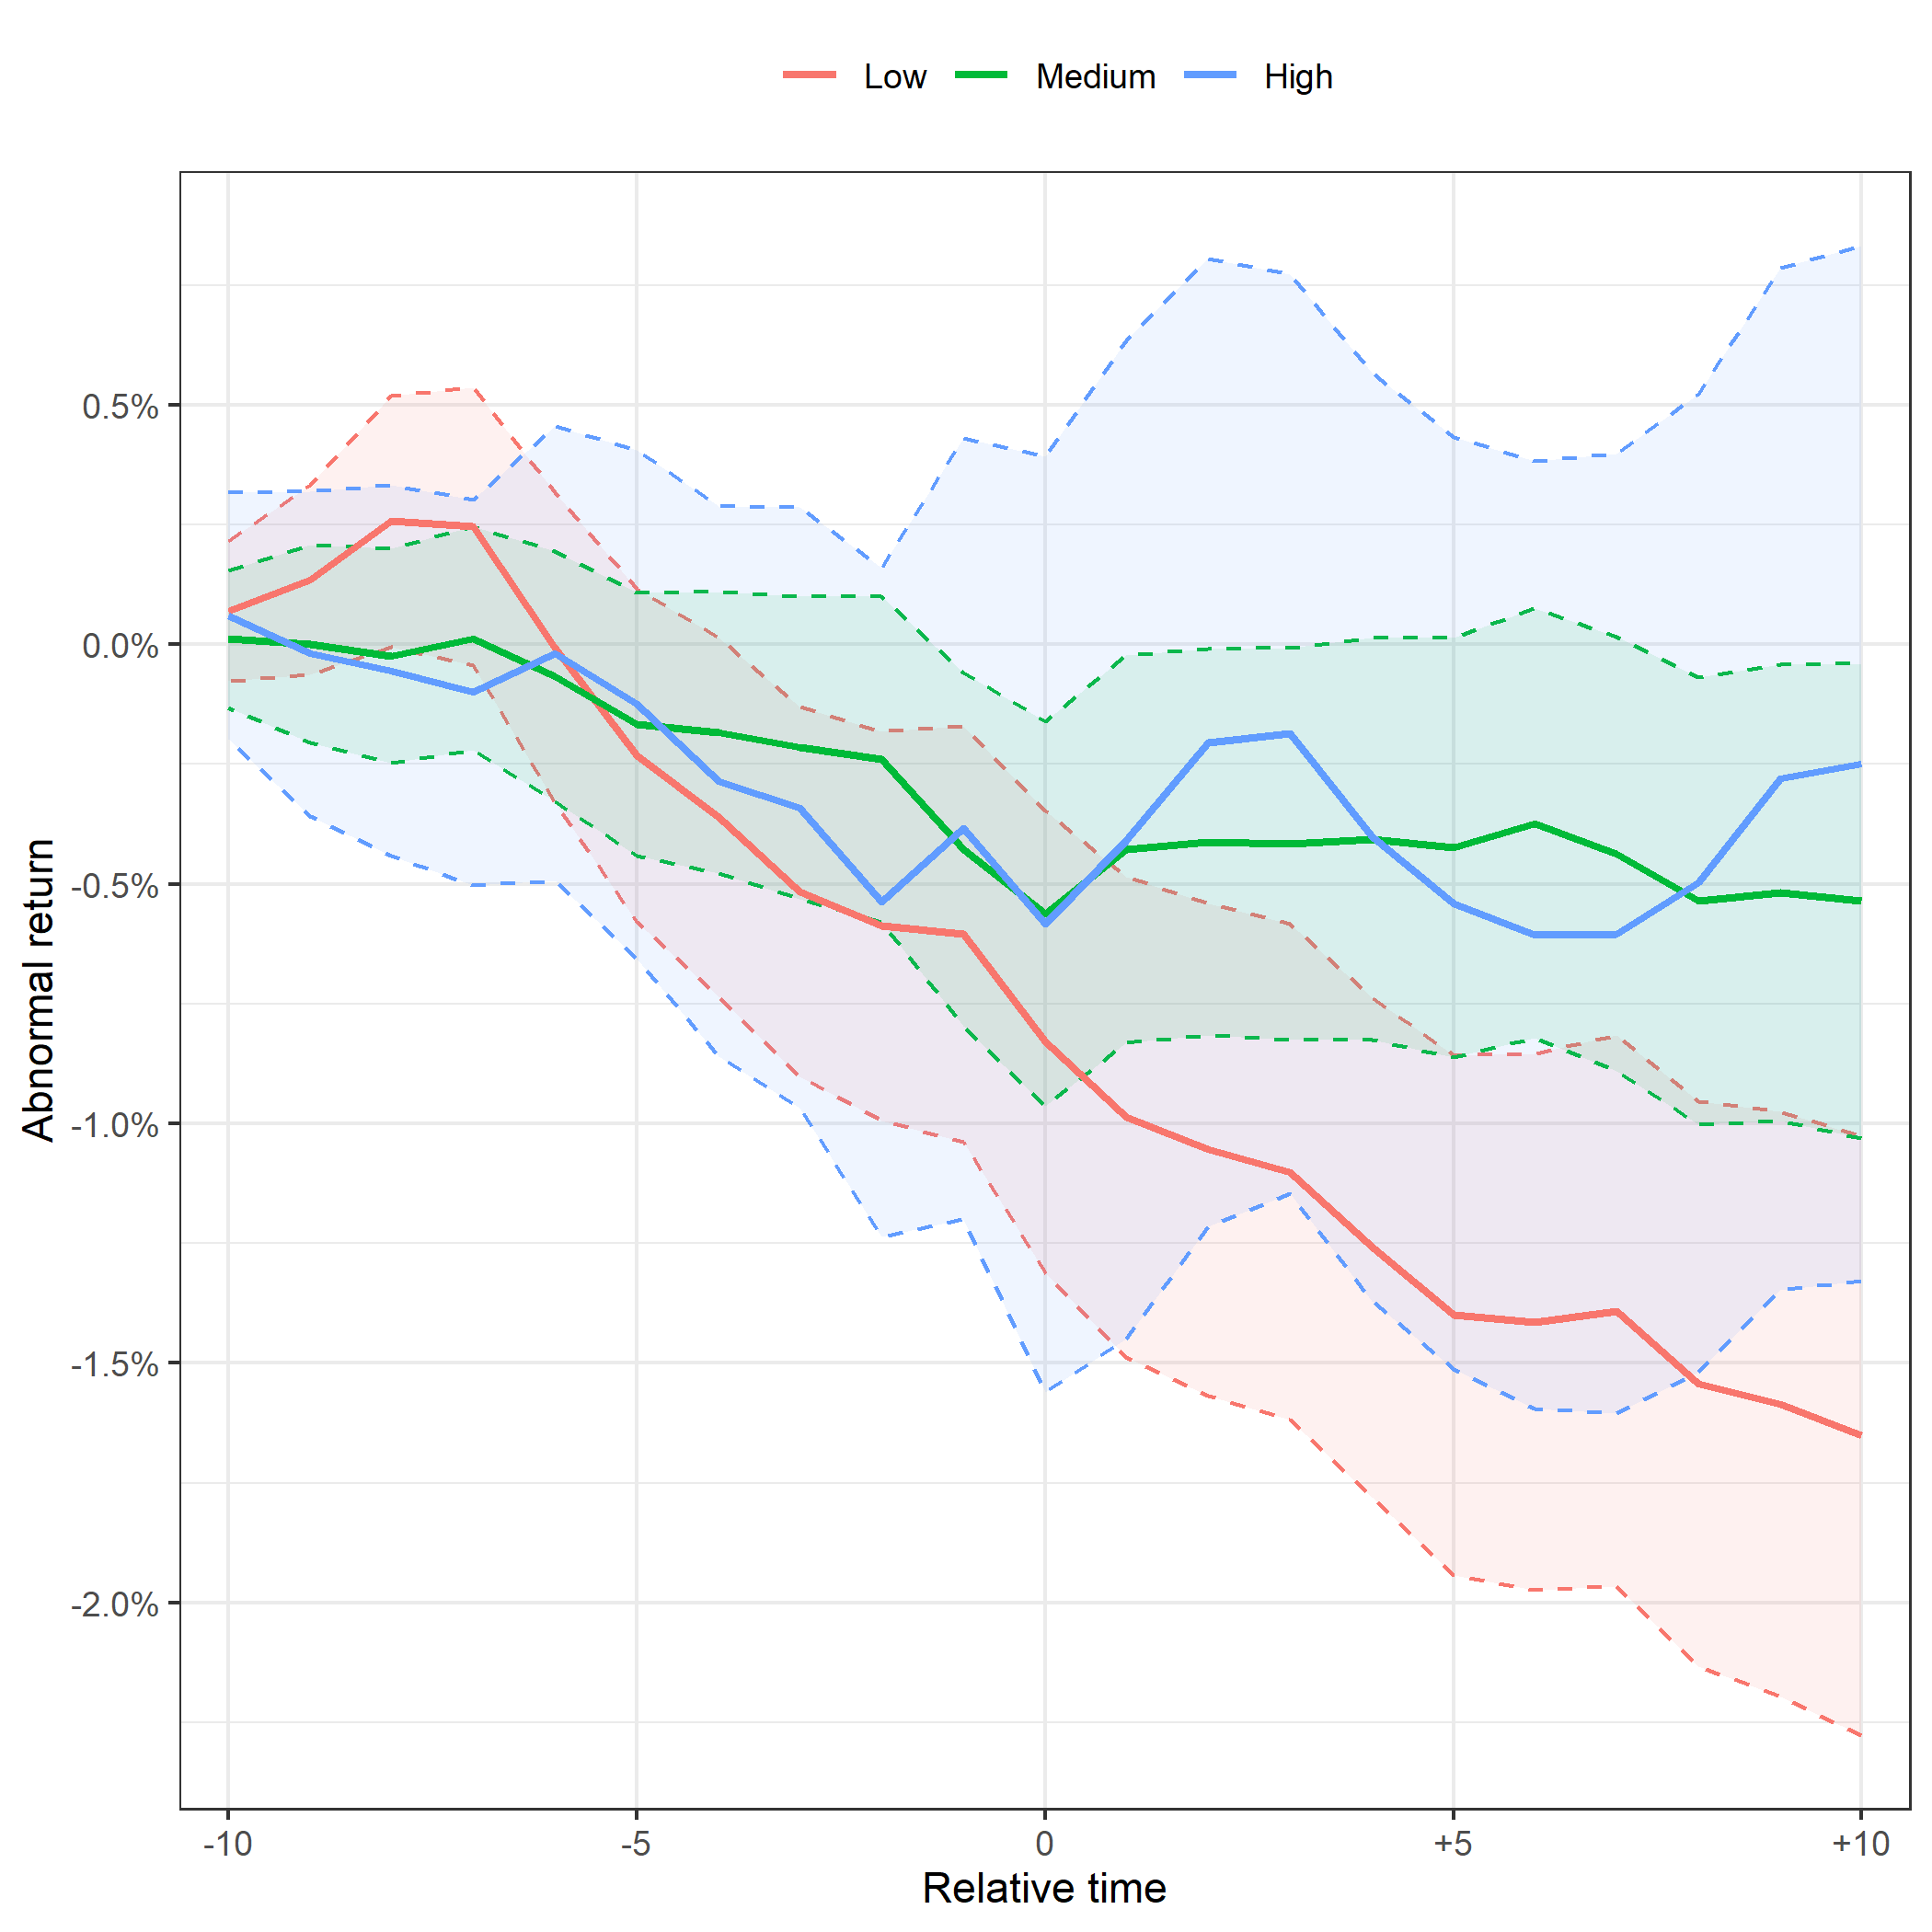
\includegraphics[scale=0.6]{Projekt/1.Figures analysis/ST_negative_ESG.png}
     \caption*{\footnotesize The figure illustrates the CAAR around the event date of negative news. The lines represent low, medium and high ESG risk of the firms in the sample. The ribbons represent the 95th confidence intervals. The categories low, medium, and high have, respectively, 315, 559, and 170 observed events in the sample. }
    \label{fig:ST_neg_ESG}
\end{figure} 


The CAAR of the three groups behave in dissimilar patters, indicating that the general results of negative abnormal results from figure \ref{fig:ST_neg_news} doesn't apply to all risk types.
Nonetheless, firms with low and medium risk profiles both develop significant negative abnormal returns. "Low" firms are experiencing large return declines of up to 4\% after negative events, while firms with a medium profile end up at -1.1\%. As the group of high risk companies consists of only 170 observed events, the confidence intervals become wide with a mean around 0\% and no significant relation can be determined. 



\subsubsection{Positive news}

The average abnormal return for positive news with the market model is marginally significant at 0.08\% on the 5\% level on the event date. According to figure \ref{fig:ST_pos_news} the remaining days of the event window are not associated with a significant reaction from shareholders. Following, the statistical uncertainty of the CAAR becomes more widespread through the event window, as indicated by the widening red ribbon. The positive tendency of the CAAR is insignificant since the measure is based on insignificant AARs, meaning that one cannot for certain state that the cumulative return is different from zero. Nonetheless, a positive reaction is inferred at $t=0$ indicating that investor do react instantly to positive news on average, however the gains seems to be depleted in the following weeks.  

\begin{figure} [H] 
    \centering
    \caption{Short term positive news: AAR and CAAR}
    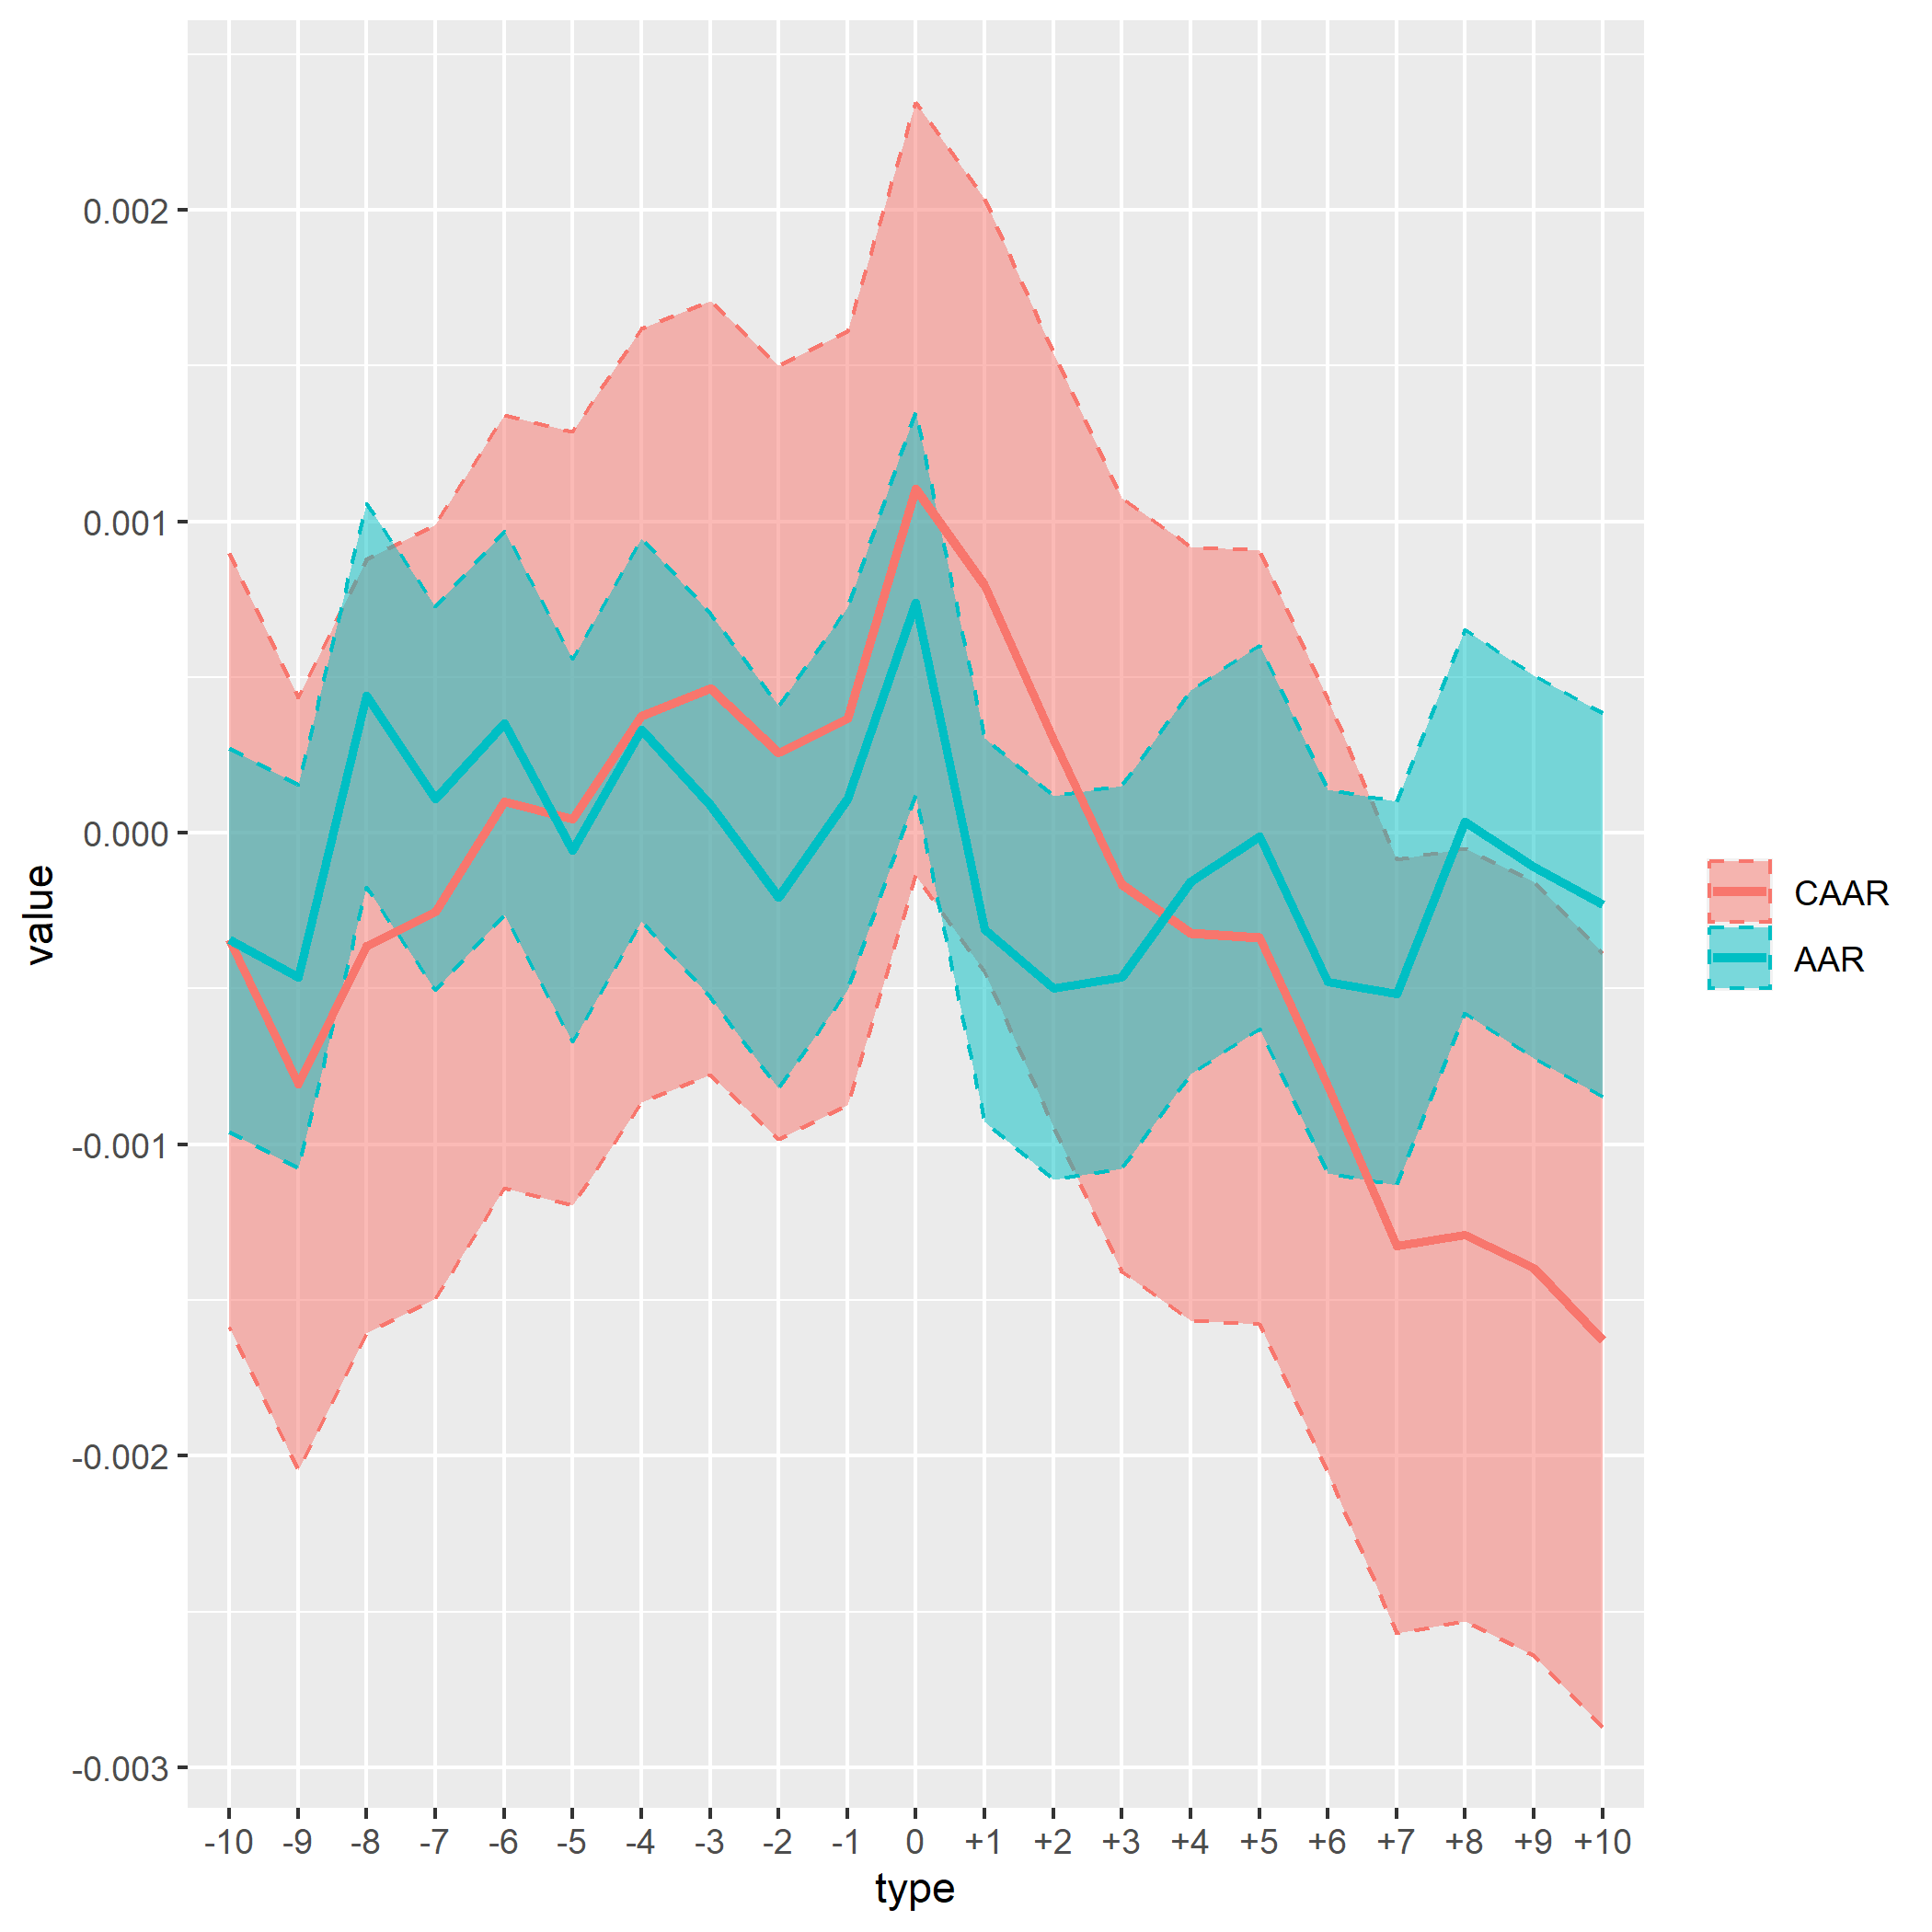
\includegraphics[scale=0.6]{Projekt/1.Figures analysis/ST_positive_all_CI.png}
    \caption*{\footnotesize The figure illustrates the average abnormal return (AAR) and cumulative AAR (CAAR) around the event date (t = 0) of positive news. The lines (left axis) represent the average and the ribbons represent the 95th confidence intervals. The bars (right axis) represent the amount of events on a given day relative to t = 0. }
    \label{fig:ST_pos_news}
\end{figure}

The insignificance of the abnormal returns associated with positive events are manifested in table \ref{tab: ST_neg_significance}. The the CAARs on, respectively, two, five and 10 days around the event are all insignificantly different from zero. However, the AAR does exhibit positive performance at $t = 0$ at 5\% significance.


\textbf{Split news on SDGs.}
The tendency of insignificance related to positive events is further emphasized by the results from the Five Pillars of SDGs, as the CAAR are not statistically different from from zero. In contrast to the case of negative events, where a potential issue was the low amount of observations, the underlying uncertainty arises from the seemingly random shareholder reaction to positive events, as indicated by the aggregate overview in figure \ref{fig:ST_pos_bar}. People, Peace, and Partnership present negative abnormal returns, while Planet and Prosperity are positive. However, none of them are significant at a 5\% level. Only SDG 7, that deals with clean energy, displays a significant, positive abnormal return as presented in the appendix \ref{fig:ST_pos_bar_all}. 

\begin{figure} [H]
    \centering
    \caption{SDG 5 pillars: positive news}
    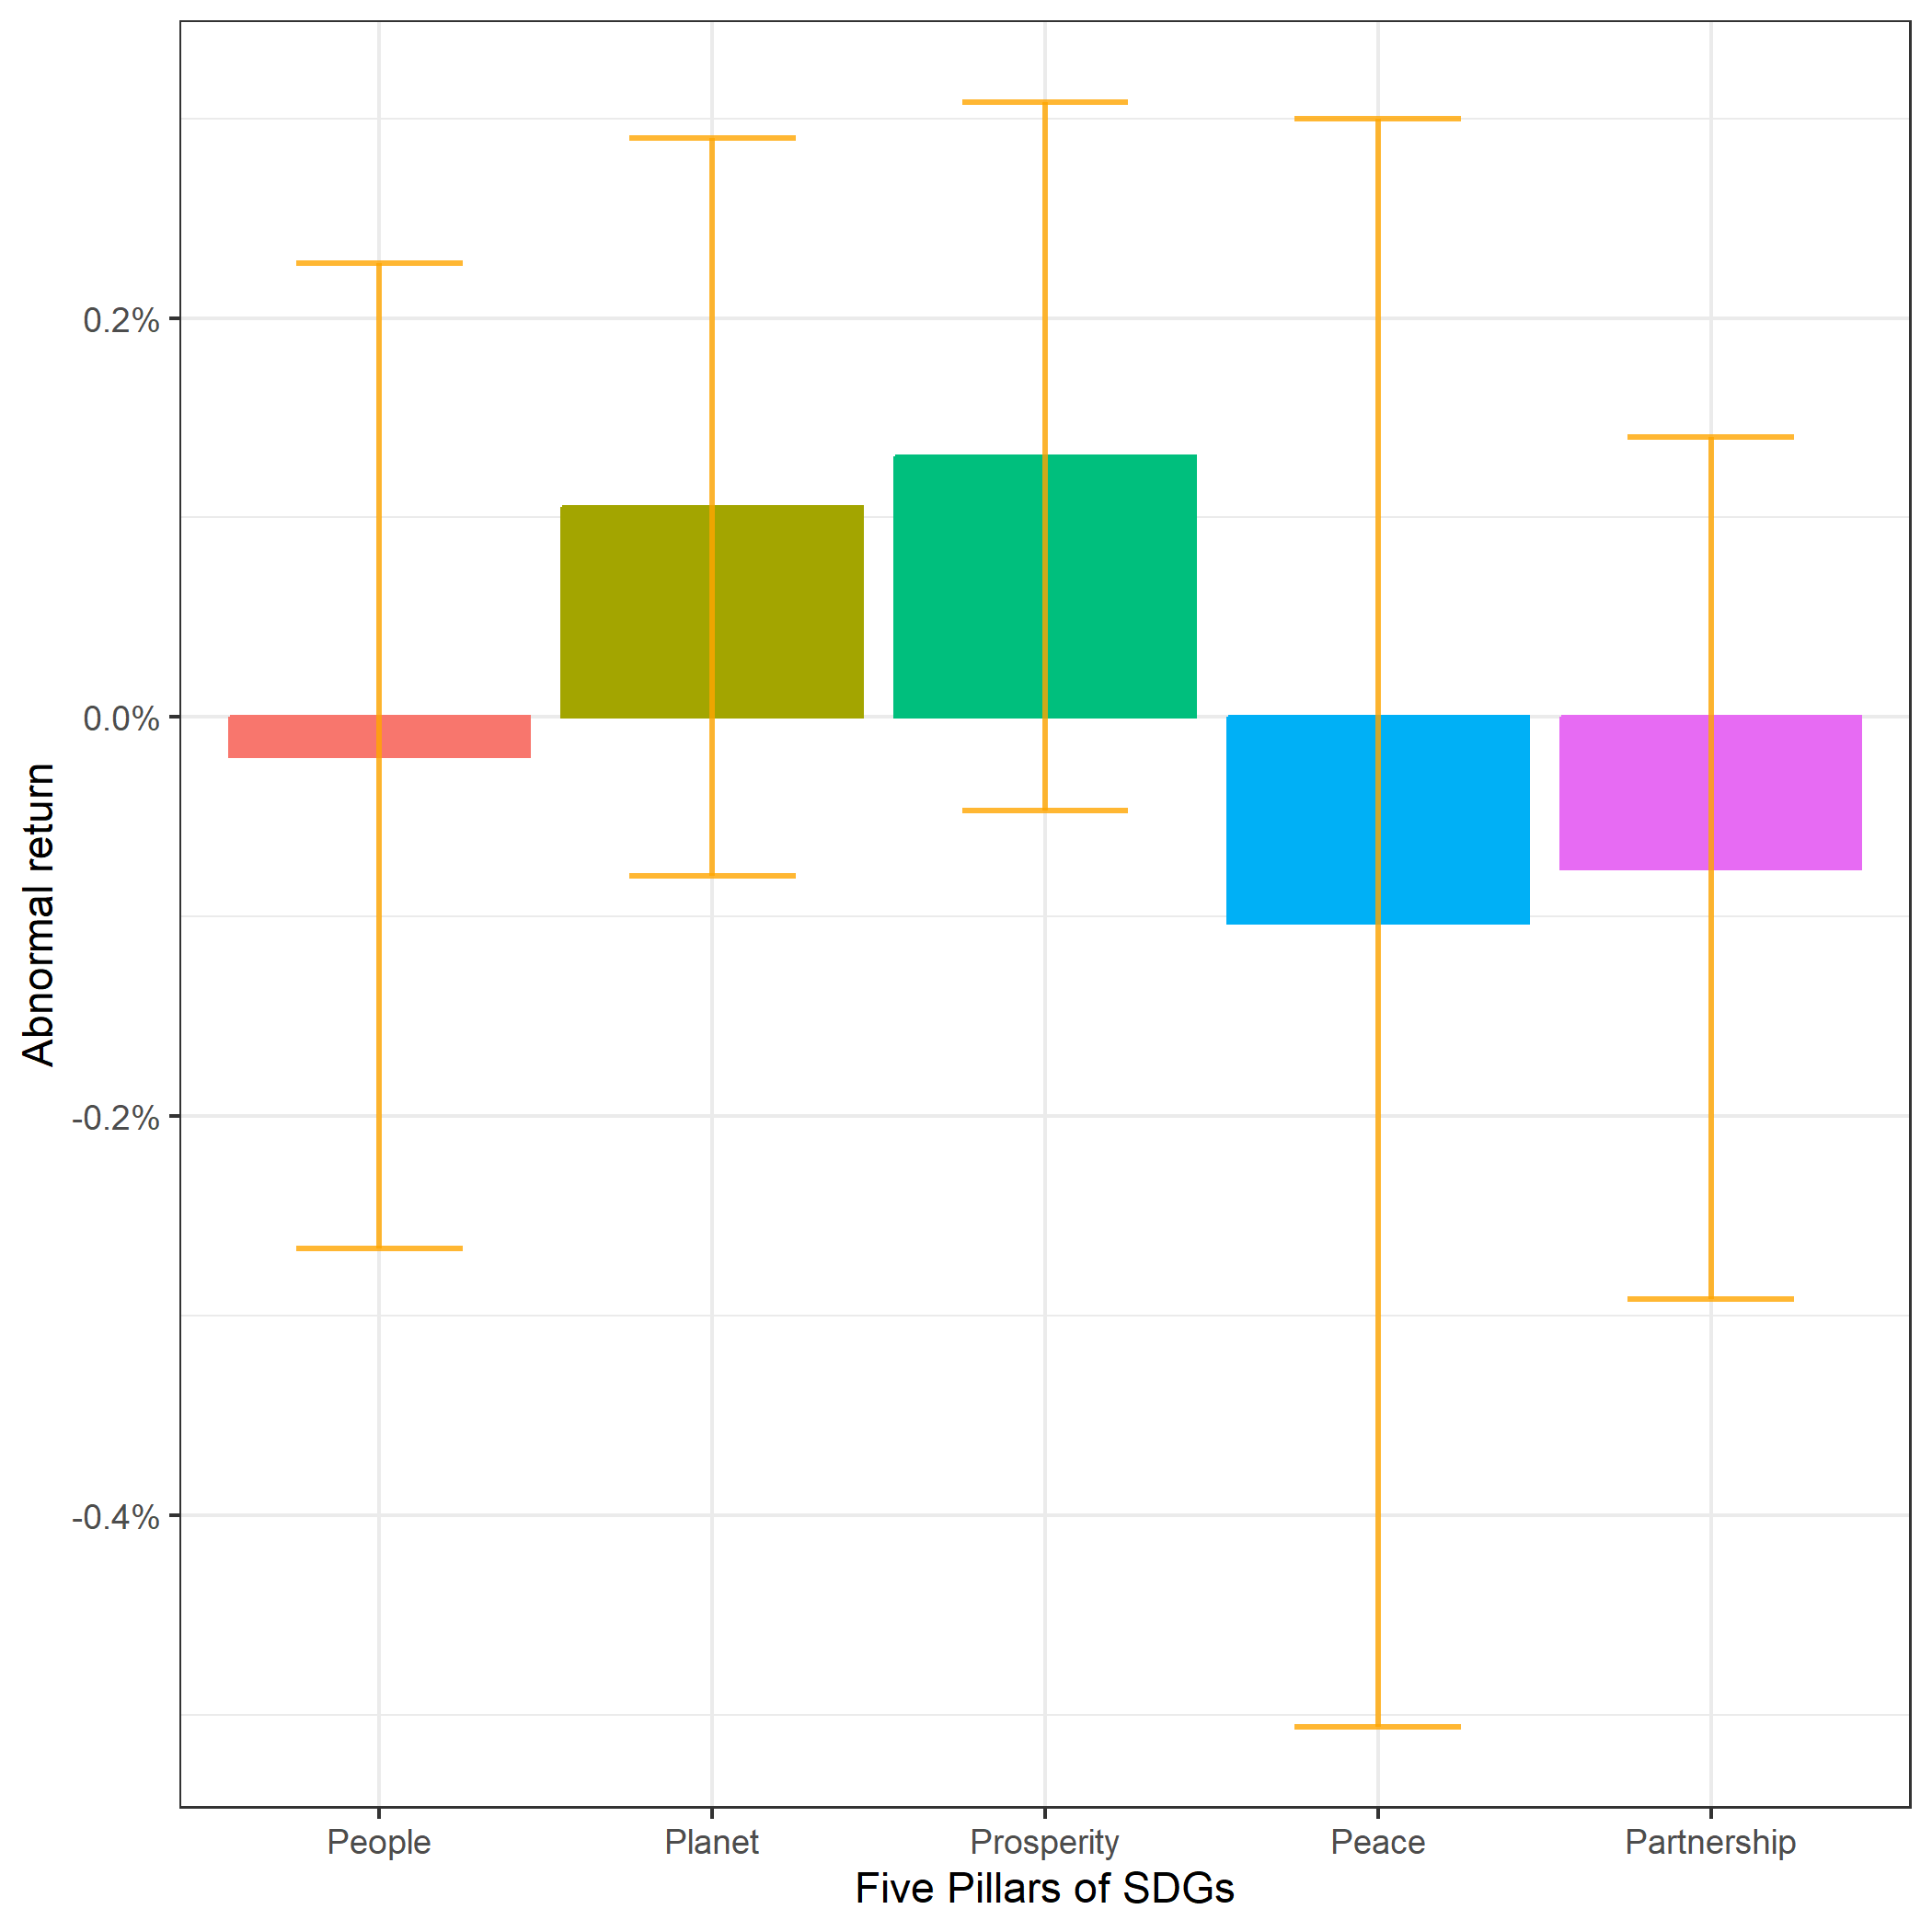
\includegraphics[scale=0.6]{Projekt/1.Figures analysis/ST_positive_sdg_bar_groups_0.png}
    \caption*{\footnotesize The figure illustrates the CAAR on $t = 10$ (full period) from positive news. The error bars represent the 95\% confidence intervals of the CAAR.}
    \label{fig:ST_pos_bar}
\end{figure}


\noindent \textbf{Split firms on ESG rating.}
In the initial results from figure \ref{fig:ST_pos_news}, the CAAR were close to zero and estimated with large uncertainty. However, an average result like such doesn't report the full narrative as an evident difference between firms with a low and medium ESG risk profile is illustrated in figure  \ref{fig:ST_pos_ESG}. Allegedly, investors are pessimistic when low ESG risk-firms are involved in positive interactions with SDGs. The CAAR is significantly negative with an average of $-0.5\%$ over the full window. High ESG risk-firms experience an average negative return of approximately the same magnitude as low risk, although the result is highly insignificant. The insignificance is partly a feature of the relatively low amount of observations. In contrary, firms with a medium risk rating enjoy a significant, positive CAAR at $0.5\%$ over the full window. 

\begin{figure} [H]
    \centering
    \caption{Positive news: CAAR split on ESG rating}
    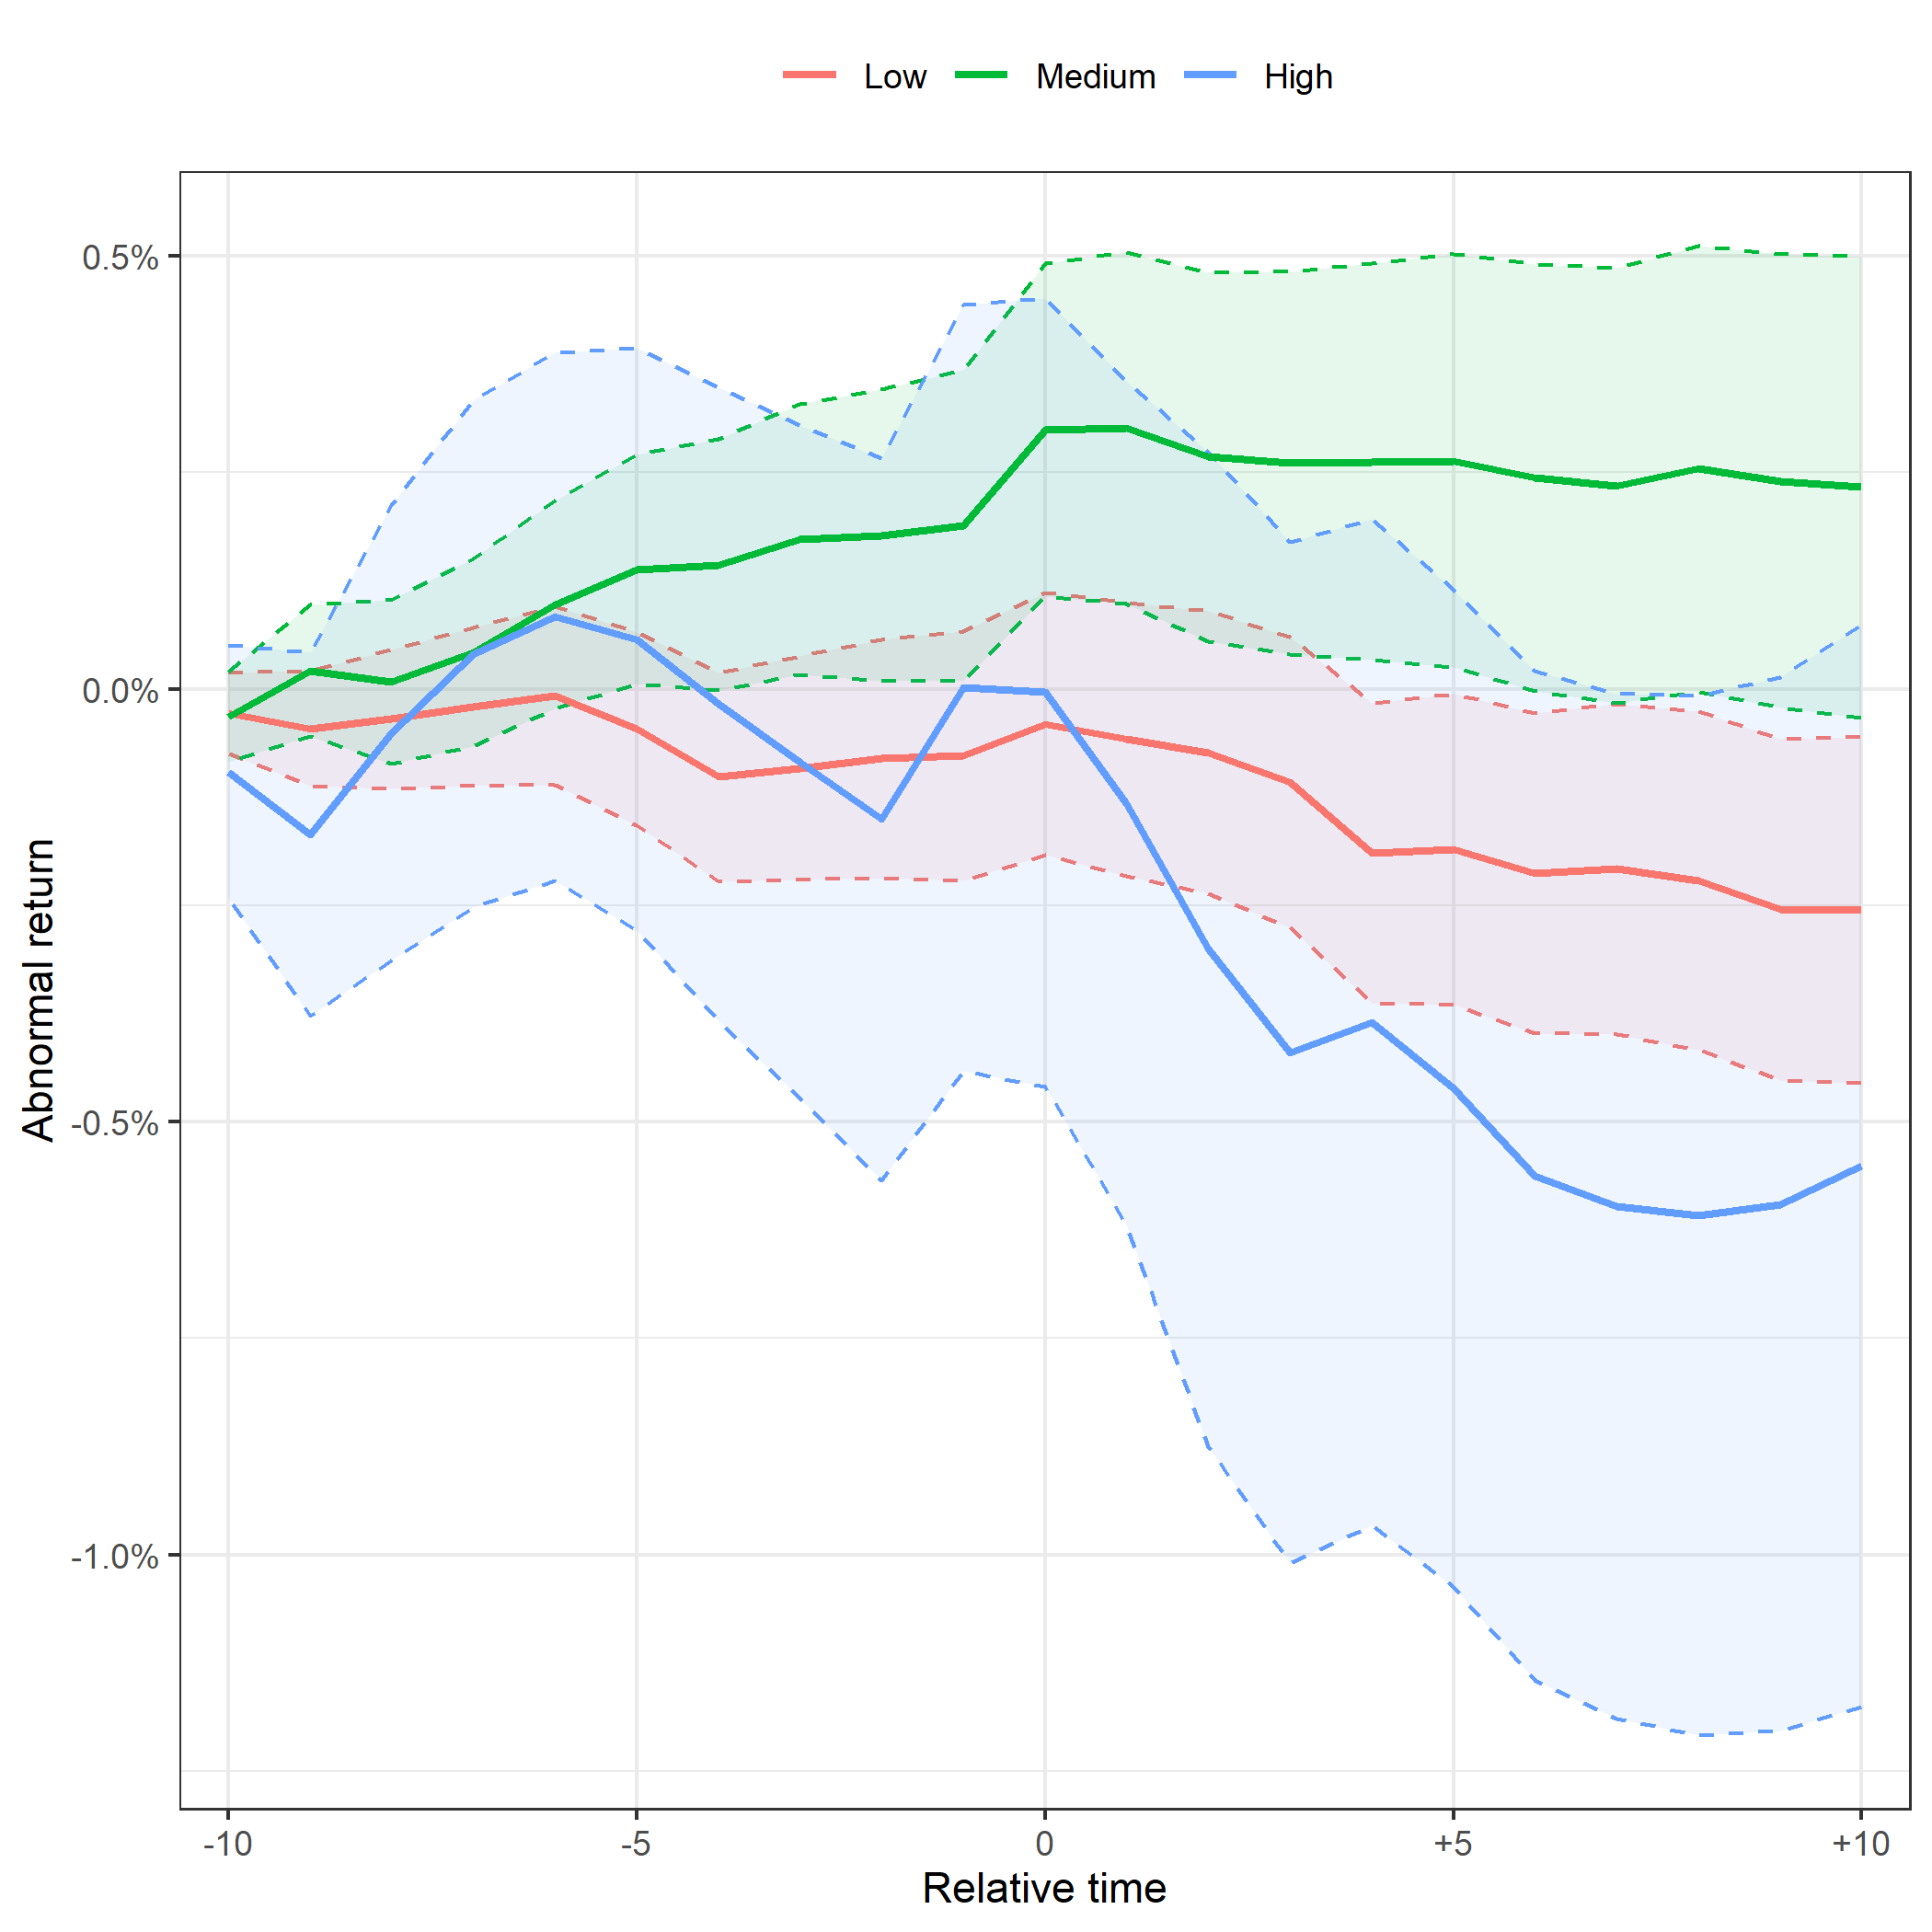
\includegraphics[scale=0.6]{Projekt/1.Figures analysis/ST_positive_ESG.png}
     \caption*{\footnotesize The figure illustrates the CAAR around the event date of positive news. The lines represent low, medium and high ESG risk of the firms in the sample. The ribbons represent the 95th confidence intervals. The categories low, medium, and high have, respectively, 1193, 1982, and 350 observed events in the sample.  }
    \label{fig:ST_pos_ESG}
\end{figure} 

Generally, the short term empirical evidence demonstrate a non-verifiable relation between positive events, related to both broad and specific SDGs, and abnormal returns. Positive news is however associated with an instant reaction from investors on the event date. Partitioning firms with regard to their ESG risk rating indicates that firms with medium risk rewarded for positive news while low and high are sold off.     



\subsection{Long term abnormal returns: The Calendar Time Portfolio} \label{sec: long_term_portfolio}

In contrast to the short term models, where the returns are measured relative to an event date, the long term portfolios are rebalanced each month and includes all firms, that have experienced an event within the T = 1/4/8/12 preceding months. The strategy resembles that T becomes the holding period for event firms. The portfolio returns are estimated over the full sample period of five years, and are evaluated by a regression on the market excess return and the factors from the Fama-French \citeyear{Fama_french_3fac} five-factor model using White heteroskedastic-robust standard errors. Moreover, any evidence of autocorrelation in all models' residuals has been rejected by a Breusch-Godfrey test of first-order. Full regression statistics including coefficient estimates, r-squared, and standard errors are available in Appendix X.  The factor models do generally have high power in explaining the excess return risk exposure, with a r-square coefficient between 73\% to 98\% throughout the various portfolios. The portfolios which hold the least amount of firms on average generally has the lowest r-squared, which generally is a result of increased variance with less observations. The long term analysis will not include a division of news depending on which SDG the news are related to, since the monthly amount of firms in the portfolios would decrease to an extent where no intuition can be drawn from the results.   


\subsubsection{Negative news}

The abnormal returns from the individual portfolios are reflected through the regression intercept from the Fama-French model, presented as the Alpha in table \ref{tab: FF3-neg} along with the corresponding t-value. The table include the mean monthly number of firms in each portfolio as "N". Moreover, the conditional event specifications are partly disclosed as the 1, 2 and 3 "SD" gives the required number of standard deviations larger than the mean for an event to be identified as consequential and thus the firm selected to the portfolio. Above each horizontal line, the "$T = x$" express the portfolio holding period after an event has occurred. 

In the matter of negative events the alphas are negative for all portfolio specifications, which indicates that the event selection methodology works as intended. However, the alphas are only significant in three instances. With a 1 SD requirement the alpha is significant for holding periods of $T = 1$ and $T = 4$ months at, respectively, -0.84\% at a $1\%$ level and -0.36\% at $5\%$. The portfolio with a 2 SD requirement and a $T=4$ holding period has significant alpha of -0.45\% at $5\%$. The alphas for holding periods larger than $T = 4$ are closer to zero and insignificant, which is in support of market efficiency over the long term. An implication of the strategy is that portfolios with longer holding periods will accordingly include more firms in each rebalancing, which ultimately will drive the portfolio return closer to the market return. For example with 1 SD, we see the inverse relation between the increases in the average N and the correspondingly decreases in alpha. In contrast, a higher SD requirement is equivalent to a more strict selection procedure designating that fewer firms will enter the portfolio. A consequence of the strict requirements is the size of the portfolios. A portfolio consisting of 5 or 10 firms will inevitably be exposed to idiosyncratic risks from the individual companies, which means that the portfolio outcome may be driven by specific risks rather than the effect from negative news. This effect is clear from the portfolio with $SD = 3$ and $T=1$, which generates an alpha of -0.78. As the alpha is relatively negative, one would expect that it would be significant as well, but the low amount of firms clearly brings too much variance into the model for the regression to be able to explain it. A large portfolio consisting of, e.g., 60 firms will not encounter the same risks due to diversification benefits. Diversification of random firms with monthly rebalancing is exactly the purpose of an exercise like this, since it allows to approximately isolate the effect of negative news from stock returns. 



Overall, the relation between negative news and returns are most severe within 1-4 months after an event has occurred and with a "loose" selection criteria of 1 SD for event firms to be included in the portfolio. Although most of the alphas are insignificant it is important to note that all are negative, which support the relation between negative news and pessimistic investor behavior.  
??. 



\textbf{Split on ESG risk profiles}
To assess whether the degree of sustainability of firms are determinants of how abnormal returns perform after encountering negative news, I estimate the portfolios with a partition on company ESG risk ratings. The results are illustrated in table \ref{tab: FF5_neg_ESG}. Similar to the original results, most alphas are negative, which indicate that the initial inference is correct. Firm characteristics of low and medium type generate alphas of approximate magnitude, however slightly lower than the overall levels from table \ref{tab: FF3-neg}. The only significant alpha is generated from firms with low ESG risk and with a portfolio holding period of one month. Such a strategy generates an abnormal return of $-0.64\%$, which is significant at the $5\%$ level with a t-statistic of -2.01. The equivalent portfolio with medium-type firms generates $-0.61$ alpha, which is high at an absolute level, however insignificant. The portfolio with high ESG risk firms and holding periods of one and four months generates considerably higher alphas of, respectively, $-2.3\%$ and $-0.93\%$. The levels are severe and would be expected to be significant. However, the amount of firms with high ESG risk is low, which directly influence the amount of firms the portfolio necessarily can hold. As the monthly average amount of firms is only two and four for the two portfolios, the returns will be exposed to idiosyncratic firm risks and determined greatly by individual company returns, which means that the factor models may have difficulties explaining the returns. Ultimately, this means that the r-squared of regressions the becomes very low at 0.4 and 0.53, which is a determinant of the low ability of generating significant alphas. 

In general, all ESG types are capable of generating negative alphas. However, only firms with low ESG risk generate a significant output on average. The outcomes are most severe and closer to being significant with shorter holding periods.   



\setlength{\tabcolsep}{15pt}
\begin{table}[H]
\small
\centering
\caption{Fama-French five-factor model alpha from negative news split on ESG risk} 
\begin{tabular}{llllllc}
\hline \hline \\ 
 &     & Overall &    Low  &  Medium  &  High &  \\    \cline{3-6} 
& &  \multicolumn{3}{c}{ T = 1} & \\ \cline{2-6}
& Alpha (\%)    & -0.84^{***} & -0.64^{**}  & -0.61  & -2.21 &  \\ 
& t-value   & -3.13 & -1.88 & -1.35  & -1.43 &  \\
& &  \multicolumn{3}{c}{ T = 4} & \\ \cline{2-6}
& Alpha (\%)   & -0.36^{**} & -0.23  & -0.33  &  -0.84 & \\
& t-value &   -2.29 & -1.06 & -1.28  & -1.23 & \\
& &  \multicolumn{3}{c}{ T = 8} & \\ \cline{2-6}
& Alpha (\%)    & -0.15 & -0.01   & -0.28  & -0.27 &  \\
& t-value &   -1.21 & -0.08  & -1.35 & -0.51 &  \\
& &  \multicolumn{3}{c}{ T = 12} & \\ \cline{2-6}
& Alpha (\%)    & -0.08 & -0.09  & -0.19  & 0.25 &  \\
& t-value &    -0.86 & -0.62  & -1.23 & 0.48 &  \\
\hline \hline
 \multicolumn{7}{l}{ \footnotesize $^* \; p\; <\; 0.1$, $ ^{**} \; p\; <\; 0.05$, $ ^{***} \; p\; <\; 0.01$  } \\
 \multicolumn{7}{p{12cm}}{ \footnotesize Alpha is the WLS-regression intercept (in \%) of the Fama-French 5-factor model, displayed along with the corresponding White heteroskedasticity-robust t-value. N is the average amount of firms included in the portfolio each month, and T is the portfolio holding period. The threshold for event firms to be included in the portfolio is either 1,2 or 3 "SD" (standard deviations) larger than the mean.} \\ 
 \hline
\end{tabular}
\label{tab: FF5_neg_ESG}
\end{table}




\subsubsection{Positive news}

The impact from positive news on financial performance in the long run is illustrated in table \ref{tab: FF5_pos}. The table applies the same format as table \ref{tab: FF3-neg}. Positive events have no significant impact on returns over any of the portfolio and event constructions. Nevertheless, the long run effect is predominantly negative, which appears in contrast to the short term effect, which indicate a positive, insignificant, relation. The performance is most negative when applying a brief holding period of $T=1$ and a strict event rule of $SD = 3$, which generates alpha of -0.37\%. With $T=1$ and $SD=1$ the portfolio achieves an alpha of -0.26\%.   
Such results are indicative of a pessimistic short-to-medium term investor reaction to general positive news. However, as the alphas are insignificant in all instances, the general conclusion is that there is no relation between positive news and stock returns.  

Applying holding periods longer than $T=1$ generates exclusively alphas close to zero, which resembles a well-diversified portfolio return close to the market portfolio, which is an expected result if positive news are recognized as irrelevant. Enforcing stricter event requirements by altering the amount of standard deviations doesn't change the results. Even the most positive news related to SDGs doesn't generate a positive abnormal return. 




\textbf{Split on ESG risk rating.}
Dividing the event firms into categories of low, medium or high ESG risk changes the narrative slightly. Table \ref{tab: FF5_pos_ESG} illustrates the alpha generated from the firms in such groups after experiencing a 1-standard deviation positive event. Firms with low and medium ESG risk experience a slight change in alpha, with none of the new estimates being significant. As before, most alphas are close to zero. On the contrary, firms with high ESG risk are enjoying a highly positive alpha when the look-back period is four months or higher. The alpha resulting from T = 12 is significantly positive, while the alpha of T = 4 and T = 8 are high but insignificant, although accompanied by quite high t-statistics. With T = 1 the abnormal returns are negative - on par with the short term results. 
The average monthly amount of firms in the portfolios does contribute to the distinctive results. For example, the portfolios with holding periods of one and four months keep on average two and four firms, which imply that the returns are exposed to idiosyncratic risks and may not be solely determined by the positive news-factor, as intended. The results indicate that firms with a prospect of high ESG risks are rewarded on the long horizon for drawing positive news related to SDGs.


\setlength{\tabcolsep}{15pt}
\begin{table}[H]
\small
\centering
\caption{FF-5 model alpha from positive news split on ESG risk} 
\begin{tabular}{ccccccc}
\hline \hline \\  
 &     & Overall  &    Low  &  Medium  &  High  &  \\ \cline{3-6} 
& & \multicolumn{4}{c}{ T = 1} & \\ \cline{2-6}
& Alpha (\%)  & -0.26 & -0.04  & -0.41  & -0.59 &  \\
& t-value & -1.03 & -0.12 & -1.47  & -0.47 & \\
& &  \multicolumn{4}{c}{ T = 4} & \\ \cline{2-6}
& Alpha (\%)  & -0.04 & -0.22  & -0.18  &  0.90 & \\
& t-value & -0.26 & -1.15 & -0.91  & 1.15 & \\
& &  \multicolumn{4}{c}{ T = 8} & \\ \cline{2-6}
& Alpha (\%)  & 0.01 & -0.23   & 0.03  & 1.06 &  \\
& t-value & 0.05 & 1.64  & 0.26 & 1.65 & \\
&  &  \multicolumn{4}{c}{ T = 12} & \\ \cline{2-6}
& Alpha (\%)  & 0.05 & -0.14  & 0.02  & $0.97^{*}$ &  \\
& t-value & 0.76 & -1.11  & 0.19 & 1.72 & \\
\hline \hline
 \multicolumn{7}{l}{ \footnotesize $^* \; p\; <\; 0.1$, $ ^{**} \; p\; <\; 0.05$, $ ^{***} \; p\; <\; 0.01$  } \\
 \multicolumn{7}{p{12cm}}{ \footnotesize Alpha is the WLS-regression intercept (in \%) of the Fama-French 5-factor model, displayed along with the corresponding White heteroskedasticity-robust t-values. T is the portfolio holding period. The threshold for event firms to be included in the portfolio is 1 standard deviation from the mean.}  \\ 
\end{tabular}
\label{tab: FF5_pos_ESG}
\end{table}